% =====================================================================
%  MSc Defense -- Master Deck (English)
%  Spine: data-mining -> cleaning -> target -> training -> eval -> deploy
%         framed against frontier-lab LLM engineering.
%  VERTICAL SLICE: ACT 0 (framing) + ACT 1 (data mining / CV + parallel).
% =====================================================================
\documentclass[aspectratio=169,11pt]{beamer}

\usepackage{amsmath}
\usepackage{amssymb}
\usepackage{array}
\usepackage{booktabs}
\usepackage{graphicx}
\usepackage{siunitx}
\usepackage{xcolor}
\usepackage{xurl}
\usepackage{tikz}
\usetikzlibrary{arrows.meta,shapes.geometric}
\usepackage{animate}

\usetheme{Madrid}
\usecolortheme{default}
\setbeamertemplate{navigation symbols}{}
\setbeamertemplate{footline}[frame number]
\graphicspath{{assets/}}
\urlstyle{same}

\definecolor{goodGreen}{RGB}{35,120,75}
\definecolor{warnRed}{RGB}{170,55,55}
\definecolor{aaltoBlue}{RGB}{0,83,155}
% concept-map palette (data mental-model slide)
\definecolor{cmPink}{RGB}{236,130,223}
\definecolor{cmGreen}{RGB}{140,198,94}
\definecolor{cmYellow}{RGB}{250,200,90}
\definecolor{cmGray}{RGB}{150,150,150}
\definecolor{cmRed}{RGB}{238,45,45}
\definecolor{cmPurple}{RGB}{178,60,168}
\definecolor{cmViolet}{RGB}{140,70,230}

\newcommand{\good}[1]{\textcolor{goodGreen}{#1}}
\newcommand{\warn}[1]{\textcolor{warnRed}{#1}}
\newcommand{\blue}[1]{\textcolor{aaltoBlue}{#1}}
\newcommand{\src}[1]{\vfill{\tiny\textcolor{gray!70!black}{Source: #1}}}
\newcommand{\pathtext}[1]{{\scriptsize\url{#1}}}
\newcolumntype{L}[1]{>{\raggedright\arraybackslash}p{#1}}
\newcolumntype{R}[1]{>{\raggedleft\arraybackslash}p{#1}}
\newcolumntype{C}[1]{>{\centering\arraybackslash}p{#1}}

% Recurring visual motif: the frontier-lab analogy callout.
\newcommand{\llmparallel}[1]{%
  \begin{block}{$\rightrightarrows$ Frontier-lab LLM parallel}#1\end{block}}

\title[AI Spray-Penetration Surrogate]{An AI-Driven Screening Surrogate for Spray-Wall Impingement}
\subtitle{One person, one machine, the full frontier-lab pipeline}
\author{Linan Jiang}
\institute{Aalto University}
\date{MSc Thesis Defense, 2026}

\begin{document}

% =====================================================================
\begin{frame}
  \titlepage
  \begin{center}\small\blue{Data mining $\to$ cleaning $\to$ targets $\to$ training $\to$ evaluation $\to$ deployment}\end{center}
\end{frame}

% =====================================================================
% ACT 0 -- FRAMING
% =====================================================================

\begin{frame}{The result, up front: two interchangeable solvers}
\small
The deployed screener can run \blue{either} regressor as its solver -- same inputs,
same physical output, different inductive prior. Both are reported.
\medskip

\begin{center}
\begin{tabular}{L{0.30\linewidth}R{0.16\linewidth}R{0.18\linewidth}R{0.20\linewidth}}
\toprule
Solver (uncensored CDF) & RMSE [mm] & \makebox[0pt]{$1\sigma$ cov.} & \makebox[0pt]{$2\sigma$ cov.} \\
\midrule
\good{Production MLP} (5-seed) & $4.265 \pm 0.040$ & $0.887$ & $0.989$ \\
\good{Stage-3 SVGP}           & $4.193$           & $0.716$ & $0.945$ \\
\midrule
Hiroyasu--Arai (calibrated)   & $10.261$ & -- & -- \\
Naber--Siebers (delay)        & $9.286$  & -- & -- \\
\bottomrule
\end{tabular}
\end{center}
\medskip

\good{$\approx$58\% / 54\% lower RMSE} than the Hiroyasu--Arai / Naber--Siebers physics
correlations. The MLP trades $\sim$0.07~mm of RMSE for markedly more conservative,
better-calibrated uncertainty -- the right bias for a \emph{screening} tool.
\end{frame}

% ---------------------------------------------------------------------
\begin{frame}{The thesis in one picture: a one-person frontier-lab pipeline}
\footnotesize
My contribution is not a single model -- it is borrowing, end to end, the
\blue{engineering workflow and methodology} that frontier AI labs use to build LLMs,
and applying that discipline at the scale this problem actually calls for.
\medskip

\begin{center}
\renewcommand{\arraystretch}{1.04}
\begin{tabular}{L{0.05\linewidth} L{0.40\linewidth} L{0.45\linewidth}}
\toprule
 & \textbf{This thesis (spray surrogate)} & \textbf{\blue{Frontier-lab LLM engineering}} \\
\midrule
1 & Data mining: CV + CUDA, Mie video $\to$ 1D penetration & Web-scale data acquisition (massively parallel ingest) \\
2 & Data cleaning: censoring-aware curation, 3 populations & Data curation \& quality filtering -- ``data is the moat'' \\
3 & Target construction: $A$-scale feature + $q_1$ targets & Label / target engineering + distillation targets \\
4 & Training: 3-stage MLP, knowledge distillation & Pretrain $\to$ distill $\to$ fine-tune \\
5 & Evaluation: leave-one-nozzle-out + calibration & Evals / OOD benchmarks / calibration \\
6 & Deployment: family-head \& residual adapters + GUI & Serving + deployment-time adapters / few-shot \\
\bottomrule
\end{tabular}
\end{center}
\smallskip
\begin{center}\small\blue{This deck walks these six stages -- each with its LLM-lab parallel.}\end{center}
\end{frame}


% ---------------------------------------------------------------------
\begin{frame}{Why a surrogate at all: screen, do not replace}
\small
High-fidelity routes are accurate but unaffordable for design-space sweeps:
\begin{itemize}
  \item One reacting diesel-spray LES example: \warn{$\sim$48{,}000 CPU core-hours and up to 20 days} of wall-clock for only \warn{\SI{2}{ms}} after start of injection.\footnote{\tiny Curtis, Niemeyer \& Sung (2017), as cited in the introduction.}
\end{itemize}
\medskip
\begin{block}{Positioning (from the discussion)}
\emph{``Not to supplant CFD, but to serve as a low-cost upstream screening layer\ldots an
auditable early-stage engineering screening tool to \good{narrow the design space} before
initiating higher-fidelity validation.''}
\end{block}
\end{frame}

% =====================================================================
% ACT 1 -- DATA MINING : COMPUTER VISION + PARALLEL PROGRAMMING
% =====================================================================
\section{Data mining}

\begin{frame}{Stage 1 --- Data mining: a four-lane streaming assembly line}
\small
Raw multi-hole Mie video $\to$ plume-wise 1D penetration trajectories; full archive in
\good{$\approx$\SI{28.25}{min}} --- GPU compute, a CPU thread pool, and hidden disk I/O kept busy at once.
\smallskip

\begin{center}
\resizebox{!}{0.54\textheight}{%
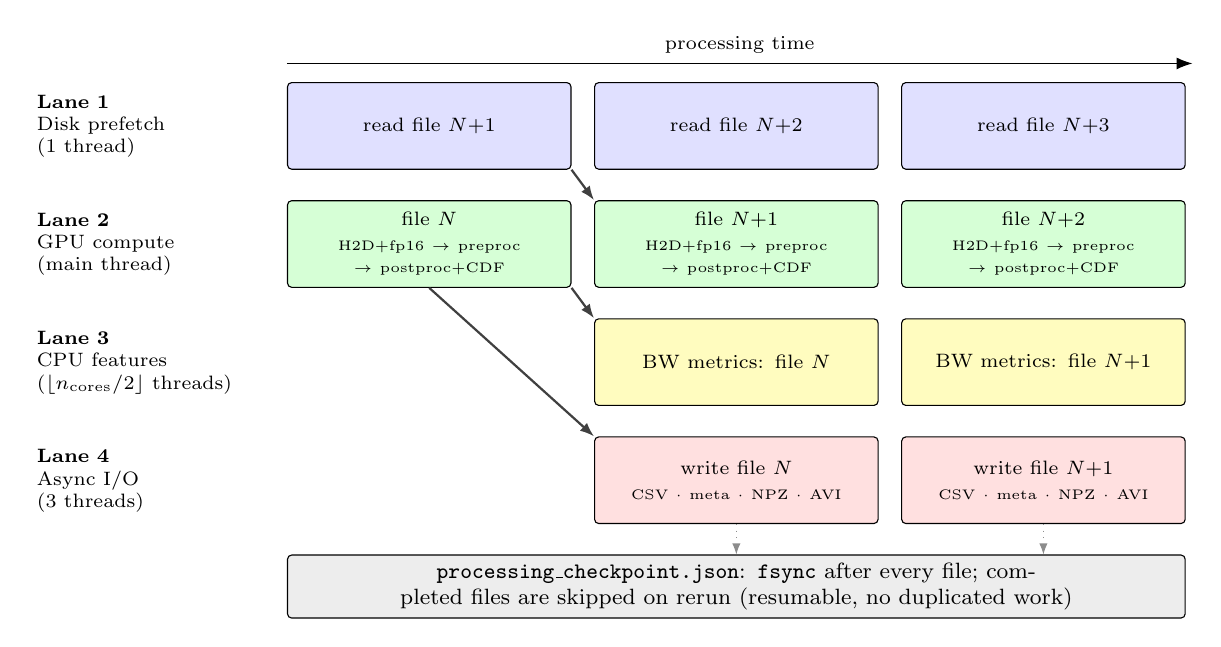
\begin{tikzpicture}[x=1mm,y=1mm,
  blk/.style={draw, rounded corners=1.5pt, align=center, font=\scriptsize, inner sep=2pt, anchor=south west},
  lbl/.style={align=left, font=\scriptsize, text width=29mm, anchor=west},
  hand/.style={-{Latex[length=1.8mm]}, thick, draw=black!75},
  ck/.style={-{Latex[length=1.4mm]}, draw=black!45, dotted},
]
% time axis
\draw[-{Latex[length=2mm]}] (33,73.5) -- (148,73.5) node[midway, above, font=\scriptsize] {processing time};
% lane labels
\node[lbl] at (0,65.5) {\textbf{Lane 1}\\Disk prefetch\\(1 thread)};
\node[lbl] at (0,50.5) {\textbf{Lane 2}\\GPU compute\\(main thread)};
\node[lbl] at (0,35.5) {\textbf{Lane 3}\\CPU features\\($\lfloor n_{\mathrm{cores}}/2\rfloor$ threads)};
\node[lbl] at (0,20.5) {\textbf{Lane 4}\\Async I/O\\(3 threads)};
% prefetch lane
\node[blk, fill=blue!12, minimum width=36mm, minimum height=11mm, text width=33mm] (pf0) at (33,60) {read file $N{+}1$};
\node[blk, fill=blue!12, minimum width=36mm, minimum height=11mm, text width=33mm] (pf1) at (72,60) {read file $N{+}2$};
\node[blk, fill=blue!12, minimum width=36mm, minimum height=11mm, text width=33mm] (pf2) at (111,60) {read file $N{+}3$};
% GPU lane
\node[blk, fill=green!16, minimum width=36mm, minimum height=11mm, text width=33mm] (g0) at (33,45) {file $N$\\[1pt]{\tiny H2D+fp16 $\to$ preproc $\to$ postproc+CDF}};
\node[blk, fill=green!16, minimum width=36mm, minimum height=11mm, text width=33mm] (g1) at (72,45) {file $N{+}1$\\[1pt]{\tiny H2D+fp16 $\to$ preproc $\to$ postproc+CDF}};
\node[blk, fill=green!16, minimum width=36mm, minimum height=11mm, text width=33mm] (g2) at (111,45) {file $N{+}2$\\[1pt]{\tiny H2D+fp16 $\to$ preproc $\to$ postproc+CDF}};
% CPU lane
\node[blk, fill=yellow!25, minimum width=36mm, minimum height=11mm, text width=33mm] (c1) at (72,30) {BW metrics: file $N$};
\node[blk, fill=yellow!25, minimum width=36mm, minimum height=11mm, text width=33mm] (c2) at (111,30) {BW metrics: file $N{+}1$};
% IO lane
\node[blk, fill=red!12, minimum width=36mm, minimum height=11mm, text width=33mm] (i1) at (72,15) {write file $N$\\[1pt]{\tiny CSV $\cdot$ meta $\cdot$ NPZ $\cdot$ AVI}};
\node[blk, fill=red!12, minimum width=36mm, minimum height=11mm, text width=33mm] (i2) at (111,15) {write file $N{+}1$\\[1pt]{\tiny CSV $\cdot$ meta $\cdot$ NPZ $\cdot$ AVI}};
% checkpoint bar
\node[blk, fill=black!7, minimum width=114mm, minimum height=8mm, text width=110mm, font=\footnotesize] (ck) at (33,3) {\texttt{processing\_checkpoint.json}: \texttt{fsync} after every file; completed files are skipped on rerun (resumable, no duplicated work)};
% handoff arrows (steady-state overlap)
\draw[hand] (pf0.south east) -- (g1.north west);
\draw[hand] (g0.south east) -- (c1.north west);
\draw[hand] (g0.south) -- (i1.north west);
% checkpoint links
\draw[ck] (i1.south) -- (i1.south |- ck.north);
\draw[ck] (i2.south) -- (i2.south |- ck.north);
\end{tikzpicture}%
}
\end{center}
\end{frame}

\begin{frame}[plain]
  \centering
  
\includegraphics[width=\paperwidth,height=\paperheight,keepaspectratio]{Multi-Hole Top-View Mie Scattering Video Processing Pipeline.png} % {mie_video_to_1d_dataflow.png}
\end{frame}
% ---------------------------------------------------------------------
\begin{frame}{The imaged subject: multi-hole injector geometry \& design space}
\small
\begin{columns}[T]
\begin{column}{0.46\linewidth}
\begin{itemize}\small
  \item Several injector families; top-view Mie captures \blue{all $N$ plumes at once} ($N=9,10,11$).
  \item Five repetitions per condition $\Rightarrow$ $45$/$50$/$55$ penetration series per condition.
  \item Hole diameter spans only $0.333$--$\SI{0.384}{mm}$ (ratio $1.15$) --- why it cannot be a standalone feature (ACT~3).
  \item This geometry defines the input space, and later the out-of-design boundary.
\end{itemize}
\end{column}
\begin{column}{0.54\linewidth}

\includegraphics[width=\linewidth,height=0.66\textheight,keepaspectratio]{nozzle_geometry_overview.png}

\includegraphics[width=\linewidth,height=0.55\textheight,keepaspectratio]{mie_decay_strip.png}
\end{column}
\end{columns}
\end{frame}

% ---------------------------------------------------------------------
\begin{frame}{CV step 0 --- Manual calibration of Nozzle center}
\small

By exploiting co-centered circular shapes of hardware and least square fitting of circles, 
we calibrate manually to find the nozzle center and px-to-mm scale for each experimental setup.

\[
x_i^2+y_i^2 + D x_i + E y_i + F = 0,
\]
which is solved via least squares using standard linear solvers (e.g., \texttt{np.linalg.lstsq}). The recovered circle parameters are:
\[
c_x=-\frac{D}{2}, \qquad c_y=-\frac{E}{2}, \qquad r=\sqrt{c_x^2+c_y^2-F},
\]
where $(c_x, c_y)$ is the nozzle center and $r$ is the fitted radius.

\end{frame}

\begin{frame}[plain]
  \centering
  
\includegraphics[width=\paperwidth,height=\paperheight,keepaspectratio]{GUI_main_interface.png}
\end{frame}

\begin{frame}[plain]
  \centering
  
\includegraphics[width=\paperwidth,height=\paperheight,keepaspectratio]{GUI_calibration_interface.png}
\end{frame}

\begin{frame}[plain]
  \centering
  
\includegraphics[width=\paperwidth,height=\paperheight,keepaspectratio]{GUI_calibration_result.png}
\end{frame}

% ---------------------------------------------------------------------
\begin{frame}{CV step 1 --- Robust log-domain background subtraction}
\small
Raw Mie intensity is corrupted by glare, vignetting and uneven illumination
(multiplicative effects). Work in log space, estimate a stable background from
pre-injection frames, then reconstruct a gated foreground.
\smallskip
\begin{columns}[T]
\begin{column}{0.50\linewidth}
\begin{align*}
L_t &= \log(V_t+\varepsilon), \quad L_{\mathrm{bkg}}=\operatorname*{median}_{t<t_{\mathrm{SOI}}} L_t,\\[2pt]
R_t &= e^{\,L_t-L_{\mathrm{bkg}}}-1 = \frac{V_t-B}{B+\varepsilon},\\[2pt]
F_t &= \max\!\big(M_t R_t - R_0 - \tau,\,0\big),
\end{align*}
with mask $M_t=\mathbf{1}[V_t>\alpha B]$.
\end{column}
\begin{column}{0.50\linewidth}

\includegraphics[width=\linewidth]{fig_mie_preproc_background.png}
\end{column}
\end{columns}
\smallskip
\good{Removes multiplicative artifacts} so plume boundaries are physically meaningful,
not illumination-driven.
\end{frame}

% ---------------------------------------------------------------------
\begin{frame}{CV step 2 --- Sobel high-pass for boundary contrast}
\small
On the clean foreground, a separable Sobel operator emphasizes liquid-phase edges
ahead of segmentation (factored into 1D smoothing + derivative passes for GPU efficiency).
\smallskip
\begin{columns}[T]
\begin{column}{0.50\linewidth}
\[
S_t=\sqrt{(K_x * F_t)^2+(K_y * F_t)^2}
\]
\[
K_x=\mathbf{g}\otimes \mathbf{d}_g,\qquad K_y=\mathbf{d}_g\otimes \mathbf{g}
\]
\smallskip
Gradient magnitude $S_t$ highlights the moving spray front while suppressing
smooth interior gradients.
\end{column}
\begin{column}{0.50\linewidth}

\includegraphics[width=\linewidth]{fig_mie_preproc_sobel.png}
\end{column}
\end{columns}
\end{frame}



% ---------------------------------------------------------------------
\begin{frame}{CV step 3a --- FFT-based plume-angle estimation}
\small
We recover the penetration axes --- how much the nozzle was rotated during installation ---
by exploiting the $P$-fold rotational symmetry of the time-summed foreground in each video.
With the calibrated center, we build the time-summed angular intensity profile $\bar{A}$ and
read the global orientation from its FFT phase at the harmonic equal to the hole count $P$.
\smallskip
\begin{columns}[T]
\begin{column}{0.38\linewidth}
\[
\hat{\phi}_0 = -\frac{\arg\!\big(\mathcal{F}\{\bar{A}\}[P]\big)}{P}\cdot\frac{180^\circ}{\pi}
\]
\[
\phi_p=\frac{360^\circ p}{P}-\hat{\phi}_0
\]
\smallskip
The $P$-th FFT harmonic recovers the absolute angular offset.
\end{column}
\begin{column}{0.62\linewidth}

\includegraphics[width=\linewidth,height=0.62\textheight,keepaspectratio]{fig_angular_occupancy.png}
\end{column}
\end{columns}
\end{frame}

% ---------------------------------------------------------------------
\begin{frame}{CV step 3b --- Affine remap into a canonical strip}
\small
Each plume is rotated and translated into a shared strip frame (nozzle at the left edge),
so all downstream geometry is rotation-agnostic and directly comparable across holes.
\smallskip
\begin{center}

\includegraphics[width=\linewidth,height=0.66\textheight,keepaspectratio]{fig_efficient_rotation.png}
\end{center}
\end{frame}

% ---------------------------------------------------------------------
\begin{frame}{CV step 4 --- CDF tip definition (robust penetration front)}
\small
Collapse each plume strip transversely into an axial profile, normalize to a CDF,
and take the front as the first quantile crossing -- robust to fractured edges and
bright speckle, unlike a brightest-pixel rule.
\smallskip
\begin{columns}[T]
\begin{column}{0.46\linewidth}
\footnotesize
\begin{align*}
H_p(t,x) &= \textstyle\sum_y I_p(t,y,x),\\[2pt]
C_p(t,x) &= \frac{\sum_{\xi\le x}\tilde H_p(t,\xi)}{\sum_\xi \tilde H_p(t,\xi)+\varepsilon},\\[2pt]
\hat{x}_p(t) &= \min\{x:\,C_p(t,x)\ge q\},\ \ q=0.995.
\end{align*}
\emph{In words:} treat axial brightness as a distribution over distance; the tip is its \textbf{99.5\% quantile} --- 99.5\% of the brightness lies behind it (a quantile, not a max, so a stray speckle can't move it).
\smallskip

\good{One scalar per plume per frame} $\Rightarrow$ the 1D penetration trajectory.
\end{column}
\begin{column}{0.54\linewidth}
\centering

\includegraphics[width=\linewidth]{penetration_td.png}
\end{column}
\end{columns}
\end{frame}

% ---------------------------------------------------------------------
\begin{frame}{CV step 4b --- Segmentation result: the detected spray boundary}
\small
Thresholding the high-pass response after morphological repair (visualization omitted here) yields a binary spray
support; its outline is the segmented plume boundary used for all downstream geometry.
\smallskip
\begin{center}

\includegraphics[width=\linewidth,height=0.68\textheight,keepaspectratio]{fig_mie_segmentation_boundary_overlay.png}
\end{center}
\end{frame}

% ---------------------------------------------------------------------
\begin{frame}{CV step 4b --- The detected boundary, in motion}
\centering
\animategraphics[autoplay,loop,controls,height=0.70\textheight]{15}{seg/seg_}{0}{99}

{\scriptsize Per-frame spray-boundary overlay --- \texttt{42\_preview.avi}, Nozzle0/T1 (injection $\to$ decay, 15\,fps loop). Animation plays in Adobe Acrobat/Reader; a static frame shows in other viewers.}
\end{frame}

% ---------------------------------------------------------------------
\begin{frame}{CUDA acceleration via CuPy $\gg$ loop execution in MATLAB (CPU)}
\small
At archive scale, a naive per-frame loop is hopeless. The pipeline is layered so the
three resources never idle:
\smallskip
\begin{center}
\begin{tabular}{L{0.16\linewidth} L{0.78\linewidth}}
\toprule
Layer & Role \\
\midrule
Backend  & One \texttt{xp} array abstraction $\to$ same code on CPU or GPU. \\
GPU      & Log-ratio, Sobel, masking, CDF reductions as batched tensor ops. \\
Geometry & Multi-hole registration into a $(P,F,H,W)$ plume tensor. \\
CPU pool & \texttt{ThreadPoolExecutor} for plume-wise metric extraction. \\
I/O      & 3-worker prefetch / write-behind hides disk behind compute. \\
\bottomrule
\end{tabular}
\end{center}
\end{frame}

% =====================================================================
% ACT 2: Data cleaning / right-censoring
% =====================================================================
\section{Data cleaning}

% ---------------------------------------------------------------------
\begin{frame}{Stage 2 --- Data cleaning: from raw records to curated populations}
\small
The cleaned archive is not one table. It splits into three derived populations, each with its own role downstream:
\smallskip
\begin{center}
\renewcommand{\arraystretch}{1.15}
\footnotesize
\begin{tabular}{@{}L{4.6cm}L{6.1cm}@{}}
\toprule
\textbf{Population} & \textbf{Size / role} \\
\midrule
\#1 Raw cleaned per-frame observations &
$\sim$\num{24316} accepted trajectories, $\sim$\num{703592} frame observations \\
\#2 Uncensored points + p50/q1 oracle &
\num{506634} points, 592 conditions; oracle covers 495 conditions, median fit RMSE \SI{0.85}{mm} \\
\#3 Per-trajectory q1 params ($\log k_{1/4}$, $\log t_0$, $\log s$) &
\num{24316} trajectories \\
\bottomrule
\end{tabular}
\end{center}
\smallskip
\llmparallel{Data curation \& quality filtering, \blue{``data is the moat''}: what you keep, and how you label it, bounds everything that trains downstream.}
\end{frame}

% ---------------------------------------------------------------------
\begin{frame}[plain]
  \centering
  
\includegraphics[width=\paperwidth,height=\paperheight,keepaspectratio]{Data_Ontology.png}
\end{frame}


% ---------------------------------------------------------------------
% Raw CV output -> sets up the two right-censoring mechanisms
\begin{frame}{Raw CV output: two ways a trajectory ends}
\small
Three penetration definitions per recording --- CDF vs.\ binary axial / polar --- all ten plumes overlaid:
\smallskip
\begin{center}

\includegraphics[width=\linewidth,height=0.32\textheight,keepaspectratio]{raw_cv_signal_loss.png}\\[-2pt]
{\scriptsize \textbf{Signal loss:} CDF (left) holds a stable plateau; the binary metrics fragment and collapse as the late-time Mie signal fades.}

\smallskip

\includegraphics[width=\linewidth,height=0.32\textheight,keepaspectratio]{raw_cv_fov_censoring.png}\\[-2pt]
{\scriptsize \textbf{FOV censoring:} all three flatten at a common $\approx$\,\SI{92}{mm} ceiling --- the spray exits the camera window, not a physical stop.}
\end{center}
\end{frame}

% ---------------------------------------------------------------------
\begin{frame}{Right-censoring I: a structural field-of-view ceiling}
\small
\begin{columns}[T]
\begin{column}{0.45\linewidth}
Top-view Mie is chosen to see all $N$ plumes at once --- the scientific payoff. The tradeoff is a finite window:
\begin{itemize}\setlength\itemsep{1.5pt}
  \item \SI{180}{mm} window (radius \SI{90}{mm}) $\Rightarrow$ only $\approx$80--85\,mm effective horizontal penetration after near-nozzle masking;
  \item even with umbrella-angle correction ($\approx$1.05--1.2$\times$), lengths stay below the wall distance of the smallest Wärtsilä W20DF (bore \SI{200}{mm}, radius \SI{100}{mm});
  \item \warn{39.6\%} of cleaned trajectories hit the FOV cap (median cap \SI{92.52}{mm}, median time-to-cap \SI{1.76}{ms}).
\end{itemize}
\end{column}
\begin{column}{0.52\linewidth}

\includegraphics[width=\linewidth,height=0.62\textheight,keepaspectratio]{fig_censor_fov_saturation.png}
\end{column}
\end{columns}
\smallskip
Verdict: a \blue{structural limitation of top-view diagnostics for real-scale cylinder-wall observation} --- not a mismatch of one specific engine.
\end{frame}

% ---------------------------------------------------------------------
\begin{frame}{Right-censoring II: late-time Mie signal decay}
\small
\begin{columns}[T]
\begin{column}{0.45\linewidth}

\includegraphics[width=\linewidth,height=0.55\textheight,keepaspectratio]{mie_decay_strip.png}
\centering\scriptsize Representative raw multi-hole Mie frames
\end{column}
\begin{column}{0.52\linewidth}
\raggedright
Even while the plume stays \emph{inside} the FOV, the Mie signal can still fail:
\begin{itemize}\setlength\itemsep{1.5pt}
  \item droplet breakup, spatial dilution, and falling droplet number density push intensity below the detection threshold;
  \item the signal becomes indistinguishable from the CV-subtracted background;
  \item onset varies by condition --- some enter signal-loss before $t<\SI{0.5}{ms}$, others survive much later, and it differs plume-to-plume.
\end{itemize}
Detection rule: smoothed per-bin trajectory count drops below a fixed fraction of its intra-condition peak.
\end{column}
\end{columns}
\end{frame}

% ---------------------------------------------------------------------
\begin{frame}{Two censoring mechanisms, one cleaning rule}
\small
\begin{columns}[T]
\begin{column}{0.49\linewidth}
\centering\textbf{\texttt{fov\_saturation}}\\[2pt]

\includegraphics[width=\linewidth,height=0.55\textheight,keepaspectratio]{fig_censor_fov_saturation.png}
\raggedright\smallskip
Spray physically exits the FOV; $p_{95}$ and the max \emph{converge} on the \SI{81}{mm} threshold.
\end{column}
\begin{column}{0.49\linewidth}
\centering\textbf{\texttt{density\_drop}}\\[2pt]

\includegraphics[width=\linewidth,height=0.55\textheight,keepaspectratio]{fig_censor_density_drop.png}
\raggedright\smallskip
Max penetration at censor onset is only $\approx$\SI{74}{mm} ($\approx$\SI{7}{mm} below threshold) --- yet trajectory count collapses just as abruptly.
\end{column}
\end{columns}
\smallskip
\good{Both are detected and removed before target fitting.}
\end{frame}

% ---------------------------------------------------------------------
\begin{frame}{Designing for redundancy: a 5\,ms horizon + q1 extrapolation}
\small
\begin{columns}[T]
\begin{column}{0.45\linewidth}
Raw observations are effectively exhausted by $\approx$\SI{2}{ms} after spatial censoring.

The q1 reconstruction --- a sigmoid-gated quarter-root single-branch reduced-order fit ---
\[
\begin{aligned}
S_{q1}(t)&=\sigma\!\left(\tfrac{t-t_0}{s}\right)k_{1/4}\,t^{1/4},\\[2pt]
\sigma(z)&=\frac{1}{1+e^{-z}},
\end{aligned}
\]
is deliberately extended to a \blue{\SI{5}{ms}} horizon for design redundancy and uniform temporal density.
\smallskip
Censoring causes severe time-bin imbalance ($\sim$\num{65000} frames/bin at $t=\SI{0.15}{ms}$ $\to$ $<200$ by \SI{1.55}{ms}); per-bin count CV \good{0.52 $\to$ 0.052} after truncation.
\end{column}
\begin{column}{0.52\linewidth}

\includegraphics[width=\linewidth,height=0.62\textheight,keepaspectratio]{fig_q1_residual_structure.png}
\end{column}
\end{columns}
\end{frame}

\begin{frame}[plain]
  \centering
  
\includegraphics[width=\paperwidth,height=\paperheight,keepaspectratio]{q1_fit_example_1.png}
\end{frame}

\begin{frame}[plain]
  \centering
  
\includegraphics[width=\paperwidth,height=\paperheight,keepaspectratio]{q1_fit_example_2.png}
\end{frame}

\begin{frame}[plain]
  \centering
  
\includegraphics[width=\paperwidth,height=\paperheight,keepaspectratio]{q1_fit_example_3.png}
\end{frame}

% =====================================================================
% ACT 3: Target construction / feature engineering
% =====================================================================
\section{Target construction}

% ---------------------------------------------------------------
\begin{frame}{Stage 3 --- Target construction: engineer the feature, let data choose the regime}
\footnotesize
\textbf{Motivation:} classical spray correlations already encode physically-motivated scaling exponents for pressure, density, and diameter; we keep that prior as a hard divisor and let the data choose \emph{which} regime's exponent actually fits the training window --- instead of re-deriving the law or trusting the asymptote blindly.

\vspace{0.3em}
\textbf{This act, in one sentence:} construct one engineered amplitude feature $A_{\mathrm{scale}}$ from $\Delta P,\rho_a,d_n$; use it to reparameterize the target $S(t)\to S(t)/A$; validate the exponent choice with data, ablation, and a collapse check.

\vspace{0.3em}
\textbf{Two uncertainties, in our context:} \emph{aleatoric} --- irreducible plume-to-plume / shot-to-shot dispersion at fixed conditions, carried by the heteroscedastic $\sigma$ head (kept deliberately over-dispersed for screening); \emph{epistemic} --- model uncertainty over thinly-sampled regions (OOD nozzle families, the extrapolated tail), reducible only with more data or trunk capacity. \blue{Feature engineering moves both:} $A$-scaling strips deterministic nuisance scale so structured variation is not read as noise (lower apparent aleatoric spread); folding $d_n$ into $A$ rather than feeding it raw blocks the nozzle-identity memorization that would fake epistemic confidence over just 6 discrete diameters.

\end{frame}

% ---------------------------------------------------------------
\begin{frame}{Physical priors meet a data-driven regression}
\begin{columns}[T]
\column{0.45\linewidth}
\small
\textbf{Physical prior} --- classical reference exponents:
\[
\Delta P^{1/4},\quad \rho_a^{-1/4},\quad d_n^{1/2}.
\]

\medskip
\textbf{Data-driven regression} --- re-estimate them by an OLS log-log fit in each \SI{0.1}{ms} bin:
\[
\log S = a\,\log\Delta P + b\,\log P_{\mathrm{ch}} + c\,\log d_n + \mathrm{const}.
\]
{\footnotesize($\Delta P=P_{\mathrm{inj}}-P_{\mathrm{ch}}$, $P_{\mathrm{ch}}\propto\rho_a$.)}\ The fitted slopes \blue{$a,b,c$ \emph{are} the exponents} --- read directly against the classical $1/4,-1/4,1/2$.

\column{0.52\linewidth}
\centering

\includegraphics[width=\linewidth,height=0.54\textheight,keepaspectratio]{time_windowed_exponents.png}

{\scriptsize Per-\SI{0.1}{ms} log-log OLS of $\log S$ on $(\log\Delta P,\log P_{\mathrm{ch}},\log d_n)$ (window $\pm\SI{0.05}{ms}$); each curve is a fitted exponent vs.\ time, shaded $=$ 95\% CI, dashed $=$ Bernoulli ($0.5$) / H--A ($0.25,-0.25$) references.}
\end{columns}

\vspace{0.3em}
\footnotesize
\textbf{What it shows} --- pressure scaling is real but \emph{time-varying} (drifts toward H--A as $t$ grows), chamber-density scaling matches H--A, and \warn{diameter is not identifiable}. The numbers, next.
\end{frame}

% ---------------------------------------------------------------
\begin{frame}{Reading the exponents: a time-binned log-log regression}
\small
\textbf{Classical laws under test.}\; Hiroyasu--Arai \& Naber--Siebers both scale as $S\propto(\Delta P/\rho_a)^{1/4} d_n^{1/2}\,t^{1/2}$ (N--S adds a $k_{NS}$ prefactor and onset shift $t\!\to\!t-\tau$). \textbf{Time-binning.} Each condition is truncated at its censor onset $\to$ near-uniform per-bin counts (count CV \good{$0.52\to0.052$}); the log-log OLS from the previous slide is fit \emph{independently} in every \SI{0.1}{ms} bin ($\pm\SI{0.05}{ms}$) on the \num{506634}-point uncensored set.

\smallskip
\begin{columns}[T,onlytextwidth]
\column{0.49\linewidth}
\centering
\footnotesize
\renewcommand{\arraystretch}{1.0}
\setlength{\tabcolsep}{4pt}
\begin{tabular}{lrrrr}
\toprule
$t$\,[ms] & $a_{\Delta P}$ & $b_{P_{\mathrm{ch}}}$ & $c_{d_n}$ & $R^2$ \\
\midrule
0.30 & 0.682 & $-0.232$ & \warn{6.02} & 0.351 \\
0.40 & \good{0.523} & $-0.247$ & \warn{4.46} & 0.392 \\
0.50 & \good{0.472} & $-0.229$ & \warn{3.06} & 0.398 \\
0.60 & \good{0.521} & $-0.189$ & \warn{2.18} & 0.418 \\
0.70 & 0.447 & $-0.153$ & \warn{1.69} & 0.354 \\
\midrule
H--A & 0.25 & $-0.25$ & 0.50 & --- \\
$k_{1/4}^{\ast}$ & \good{0.52} & $-0.23$ & \warn{0.26} & 0.27 \\
\bottomrule
\end{tabular}

{\scriptsize $^\ast$pooled per-traj.\ OLS of $\log k_{1/4}$ (\num{24316} fits); rows above: per-bin $S(t)$ (\num{506634} pts).}
\column{0.49\linewidth}
\footnotesize
\begin{itemize}\setlength\itemsep{1.5pt}
  \item $a_{\Delta P}$ holds at \good{0.47--0.52} --- the \blue{Bernoulli/orifice} value $0.5$, far above H--A's $0.25$ --- drifting toward H--A as $t$ grows.
  \item $b_{P_{\mathrm{ch}}}\approx\good{-0.23\text{ to }-0.25}$, matching H--A; $R^2\approx\good{0.35\text{--}0.42}$ (single-bin scatter large, exponents stable).
  \item $c_{d_n}=\warn{1.7\text{--}6.0}$, physically impossible $\Rightarrow$ diameter \warn{not identifiable} (6 diameters, ratio 1.15, confounded with hole count).
\end{itemize}
\end{columns}

\vspace{2pt}
{\footnotesize\textbf{Verdict:} the $k_{1/4}$ row confirms the same law ($a\!\approx\!0.5$, $b\!\approx\!-0.25$); keep $\Delta P^{0.5}\rho_a^{-0.25}$ from data, fold $d_n^{0.5}$ in as an H--A prior.}
\end{frame}

% ---------------------------------------------------------------
\begin{frame}{Why diameter is folded in, not fed raw + the amplitude feature}
\small
\textbf{Facts:} only 6 discrete hole diameters spanning \num{0.333}--\SI{0.384}{mm} (ratio 1.15, log-leverage 0.14 vs.\ 0.45 for injection pressure); diameter is confounded with hole count and umbrella angle in the design matrix $\Rightarrow$ its exponent is unidentifiable.

\textbf{Move:} retain $d_n^{0.5}$ inside the amplitude as an H--A prior instead:
\[
A=\Delta P^{0.5}\,\rho_a^{-0.25}\,d_n^{0.5}.
\]

\vspace{0.3em}
\footnotesize
\textbf{Confirmed on the production model's own coefficient} --- one pooled OLS of $\log k_{1/4}$ over all \num{24316} accepted q1 fits, $\log k_{1/4}=a\log\Delta P+b\log\rho_a+c\log d_n+\text{const}$:
\renewcommand{\arraystretch}{1.05}
\begin{center}
\begin{tabular}{C{0.20\linewidth}C{0.15\linewidth}C{0.15\linewidth}C{0.34\linewidth}}
\toprule
Predictor & Exponent & H--A ref. & Verdict \\
\midrule
$\log\Delta P$ & \good{0.52} & 0.25 & data $>$ H--A $\Rightarrow$ use $\Delta P^{0.5}$ \\
$\log\rho_a$   & \good{$-0.23$} & $-0.25$ & matches H--A \\
$\log d_n$     & \warn{0.26} & 0.50 & weak ($R^2$ 0.27), unstable $\Rightarrow$ fold in \\
\bottomrule
\end{tabular}
\end{center}
\smallskip
The $d_n$ exponent is unstable across cuts (\warn{$\sim$0} matched-pressure family, \warn{0.26} pooled $k_{1/4}$, \warn{1.7--6.0} per-time-bin) --- so $d_n^{0.5}$ is kept as a fixed H--A prior, not a fitted term.
\end{frame}

% ---------------------------------------------------------------
\begin{frame}{Ablation: the cost of getting the feature set wrong}
\begin{columns}[T]
\column{0.52\linewidth}
\centering

\includegraphics[width=\linewidth,height=0.62\textheight,keepaspectratio]{fig_sparse_diameter_interpolants.png}

\column{0.45\linewidth}
\small
\textbf{Raw diameter as input:} predicted mean undergoes \warn{5--6 gradient sign reversals per slice}, with autodiff gradient spikes $\sim\!10^4$ over a $\sim$\SI{0.05}{mm} support span --- the network memorizes nozzle identity, not physics.

\vspace{0.3em}
Under LONO: adding diameter as an independent input \warn{increases mean MAE by 4--6 mm}.
\end{columns}

\vspace{0.4em}
\small
\textbf{Conversely:} \emph{removing} the residual pressure terms hurts --- Stage-1 test MAE \(8.05\to2.91\)\,mm and Stage-2 \(9.28\to5.63\)\,mm when log-pressures are kept.

\vspace{0.2em}
\textbf{Takeaway:} fold diameter into $A$; keep pressures as residual inputs.
\end{frame}

% ---------------------------------------------------------------
\begin{frame}{Target reparameterization + collapse check}
\small
The target is learned in $A$-scaled space:
\[
\hat S(t)=S(t)/A.
\]

\begin{columns}[T,onlytextwidth]
\column{0.49\linewidth}
\centering

\includegraphics[width=\linewidth,height=0.5\textheight,keepaspectratio]{collapse_dp_exp_0p25.png}

\footnotesize $\Delta P^{0.25}$
\column{0.49\linewidth}
\centering

\includegraphics[width=\linewidth,height=0.5\textheight,keepaspectratio]{collapse_dp_exp_0p50.png}

\footnotesize $\Delta P^{0.5}$
\end{columns}

\vspace{0.3em}
\footnotesize
Median post-\SI{0.5}{ms} collapse ratio: \warn{0.378} ($\Delta P^{0.25}$) vs.\ \good{0.057} ($\Delta P^{0.5}$) --- lower = better collapse onto one curve.

\textbf{Payoff:} this feature/target choice cut the 5-seed RMSE \good{10.72 $\to$ 8.92 mm (16.8\%)} on the mode-C check.

\end{frame}

% =====================================================================
% ACT 4: Training (3-stage + KD)
% =====================================================================
\section{Training}

% ---------------------------------------------------------------------
\begin{frame}{Stage 4 --- Training: a three-stage curriculum}
\small
\begin{columns}[T]
\column{0.50\textwidth}
\textbf{Architecture:} 512--512--128 MLP, dropout \num{0.30}, $\sim$150 epochs;
heads $(\mu, \log\sigma^2, \text{onset})$; 5 seeds $\{7,17,42,99,2024\}$.

\vspace{0.3em}
\textbf{Three stages} (training data $\rightarrow$ loss):
\begin{itemize}\setlength\itemsep{2pt}\footnotesize
  \item \textbf{S1} --- \emph{representative} rows (1/condition) $\rightarrow$ MSE on $\hat S{=}S/A$ + log-var prior + shape
  \item \textbf{S2} --- all \emph{filtered} rows, warm-start from S1 $\rightarrow$ Gaussian NLL + $\mu$-anchor + shape
  \item \textbf{S3} --- raw CDF series + S2 teacher $\rightarrow$ regime raw-NLL + KD$(\mu,\sigma)$ + shape
\end{itemize}

\column{0.48\textwidth}
\centering

\includegraphics[width=\linewidth,height=0.56\textheight,keepaspectratio]{mlp_architecture_overview.png}
\end{columns}

\vspace{0.2em}
{\scriptsize Shared shape penalties $P_{d1}$ (monotone front) / $P_{d2}$ (gated-concave); explicit per-stage losses on the next three slides.}

\vspace{0.2em}
\llmparallel{Exactly the frontier recipe: pretrain $\to$ distill $\to$ fine-tune, run as a
staged curriculum rather than one monolithic fit.}
\end{frame}

% ---------------------------------------------------------------------
% [COMPRESSED] Stages 1/2/3 merged into one table slide (was 3 slides:
% "Stage 1 validation: leave-one-nozzle-out feature ablation",
% "Stage 2: an early-time physics anchor stabilizes OOD",
% "Stage 3: raw-CDF refinement with regime-aware supervision").
% Per-rank ablation tables / regime-trigger tables dropped to backup if needed.
\begin{frame}{Three training stages, compressed: data, loss, purpose}
\footnotesize
\renewcommand{\arraystretch}{1.5}
\begin{center}
\begin{tabular}{@{}C{0.7cm}L{3.3cm}L{5.0cm}L{3.6cm}@{}}
\toprule
& \textbf{Data} & \textbf{Loss} & \textbf{Purpose} \\
\midrule
\textbf{S1} &
Representative rows (1/condition), $A$-scaled $\hat S{=}S/A$ &
\resizebox{4.9cm}{!}{$\mathcal{L}_1{=}\mathrm{MSE}(\hat\mu,\hat S)+\lambda_v\mathrm{MSE}(\log\hat\sigma^2,m_0)+\lambda_{d1}P_{d1}+\lambda_{d2}P_{d2}$} &
Fit median trajectory; validate feature set (\good{best 7.46\,mm MAE}, \texttt{a\_dp050\_plus\_pressures}) \\
\midrule
\textbf{S2} &
All filtered rows (full QC set); warm-start from S1 checkpoint &
\resizebox{4.9cm}{!}{$\mathcal{L}_2{=}\mathrm{NLL}_{\text{Gauss}}(\hat\mu,\hat\sigma^2,\hat S)+\lambda_\mu A_\mu+\lambda_{d1}P_{d1}+\lambda_{d2}P_{d2}$} &
Stabilize OOD generalization via early-$t$ $\mu$-anchor (\good{Nozzle2: 19.18$\to$7.76\,mm}) \\
\midrule
\textbf{S3} &
Raw empirical CDF series + S2 teacher; regime-aware by coverage (reliable/uncertain/teacher-only) &
\resizebox{4.9cm}{!}{$\mathcal{L}_3{=}\text{regime-wtd raw NLL}+\mathrm{KD}(\mu,\sigma)+\lambda_\mu A_\mu+\lambda_{d1}P_{d1}+\lambda_{d2}P_{d2}$} &
Refine on raw signal via distillation from S2 teacher; \good{production model (RMSE 4.265\,mm)} \\
\bottomrule
\end{tabular}
\end{center}

\vspace{0.4em}
{\scriptsize Shared shape priors carried through all stages: $P_{d1}$ monotone front (no recoil), $P_{d2}$ gated concavity. Each stage warm-starts from the previous stage's checkpoint -- pretrain $\to$ distill $\to$ fine-tune, as a staged curriculum rather than one monolithic fit (same frontier-lab recipe noted on the previous slide).}
\end{frame}


% =====================================================================
% [NEW] Dataset lineage diagrams (TikZ), inserted as a visual companion
% to the compressed Stage 1/2/3 table above. Definitions per thesis
% Ch.4 sec:cdf-populations-en / sec:three-derived-populations-en.
% =====================================================================
\begin{frame}{Where the training data comes from: three populations, one archive}
\centering
\resizebox{!}{0.50\textheight}{%
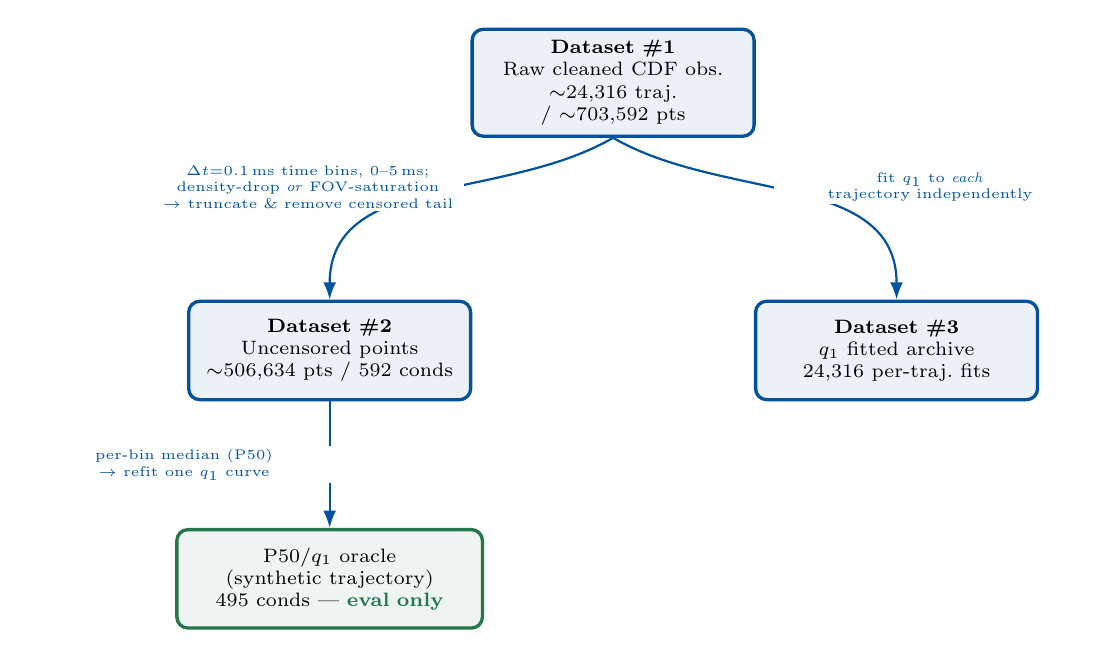
\begin{tikzpicture}[
  font=\scriptsize,
  box/.style={draw=aaltoBlue, very thick, rounded corners, fill=aaltoBlue!8,
              align=center, text width=3.3cm, minimum height=1.25cm, inner sep=4pt},
  oraclebox/.style={draw=goodGreen, very thick, rounded corners, fill=goodGreen!8,
              align=center, text width=3.6cm, minimum height=1.25cm, inner sep=4pt},
  lbl/.style={font=\tiny, align=center, text width=3.9cm, fill=white, inner sep=1pt},
  arr/.style={-{Latex[length=2.2mm]}, thick, aaltoBlue}
]

\node[box] (d1) at (4.6,6.0)
  {\textbf{Dataset \#1}\\Raw cleaned CDF obs.\\$\sim$24{,}316 traj.\ /\ $\sim$703{,}592 pts};

\node[box] (d2) at (1.0,2.6)
  {\textbf{Dataset \#2}\\Uncensored points\\$\sim$506{,}634 pts\ /\ 592 conds};

\node[box] (d3) at (8.2,2.6)
  {\textbf{Dataset \#3}\\$q_1$ fitted archive\\24{,}316 per-traj.\ fits};

\node[oraclebox] (oracle) at (1.0,-0.3)
  {P50/$q_1$ oracle\\(synthetic trajectory)\\495 conds --- \textbf{\textcolor{goodGreen}{eval only}}};

\draw[arr] (d1.south) to[out=210,in=90] node[lbl,midway,xshift=-1.55cm,yshift=0.1cm]
  {$\Delta t{=}0.1$\,ms time bins, 0--5\,ms;\\density-drop \emph{or} FOV-saturation\\$\to$ truncate \& remove censored tail} (d2.north);
\draw[arr] (d1.south) to[out=-30,in=90] node[lbl,midway,xshift=1.7cm,yshift=0.1cm]
  {fit $q_1$ to \emph{each}\\trajectory independently} (d3.north);
\draw[arr] (d2.south) -- node[lbl,midway,xshift=-1.85cm]
  {per-bin median (P50)\\$\to$ refit one $q_1$ curve} (oracle.north);

\end{tikzpicture}%
}

\vspace{0.2em}
{\scriptsize Three structurally distinct populations read from the \emph{same} cleaned CDF archive (Ch.~4, ``Right-Censoring \dots Three Derived Data Populations''). \warn{Dataset \#3 branches directly off Dataset \#1} --- it does \emph{not} pass through Dataset \#2. The P50/$q_1$ oracle is never trained on; it is the reference curve behind the ``Q1 extrapolated'' / LONO evaluation protocols.}
\end{frame}

% ---------------------------------------------------------------------
\begin{frame}{Where the training data goes: feeding Stages 1/2/3}
\centering
\resizebox{!}{0.50\textheight}{%
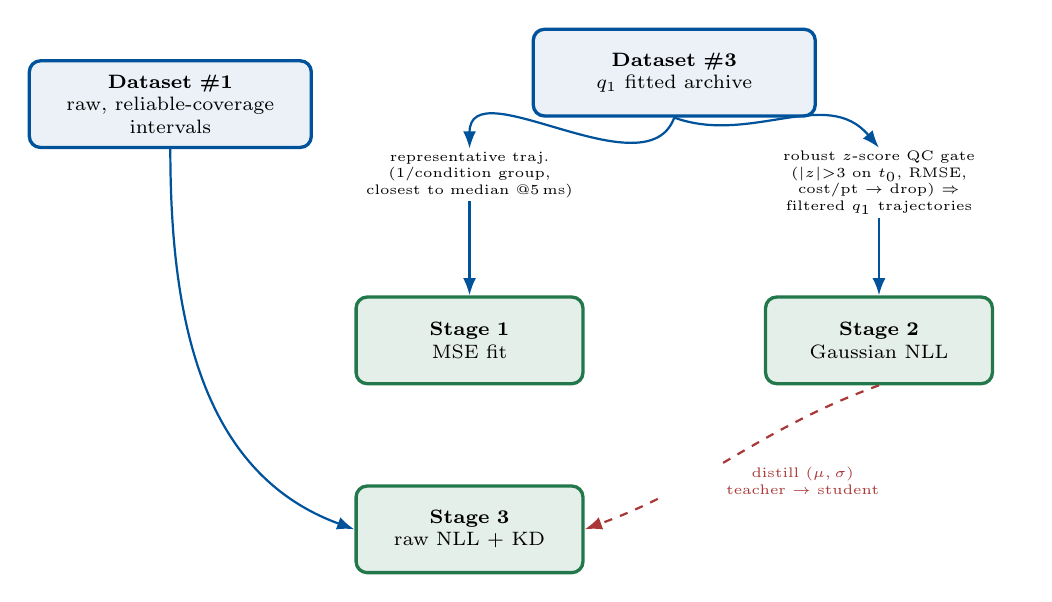
\begin{tikzpicture}[
  font=\scriptsize,
  box/.style={draw=aaltoBlue, very thick, rounded corners, fill=aaltoBlue!8,
              align=center, text width=3.3cm, minimum height=1.1cm, inner sep=4pt},
  stagebox/.style={draw=goodGreen, very thick, rounded corners, fill=goodGreen!12,
              align=center, text width=2.6cm, minimum height=1.1cm, inner sep=4pt},
  lbl/.style={font=\tiny, align=center, text width=3.6cm, fill=white, inner sep=1pt},
  arr/.style={-{Latex[length=2.2mm]}, thick, aaltoBlue},
  kdarr/.style={-{Latex[length=2.2mm]}, thick, dashed, warnRed}
]

\node[box] (d1) at (0.6,5.6) {\textbf{Dataset \#1}\\raw, reliable-coverage\\intervals};
\node[box] (d3) at (7.0,6.0) {\textbf{Dataset \#3}\\$q_1$ fitted archive};

\node[lbl] (rep) at (4.4,4.7) {representative traj.\\(1/condition group,\\closest to median @5\,ms)};
\node[lbl] (qc)  at (9.6,4.6) {robust $z$-score QC gate\\($|z|{>}3$ on $t_0$, RMSE,\\cost/pt $\to$ drop) $\Rightarrow$\\filtered $q_1$ trajectories};

\node[stagebox] (s1) at (4.4,2.6) {\textbf{Stage 1}\\MSE fit};
\node[stagebox] (s2) at (9.6,2.6) {\textbf{Stage 2}\\Gaussian NLL};
\node[stagebox] (s3) at (4.4,0.2) {\textbf{Stage 3}\\raw NLL + KD};

\draw[arr] (d3.south) to[out=250,in=90] (rep.north);
\draw[arr] (rep.south) -- (s1.north);
\draw[arr] (d3.south) to[out=-20,in=130] (qc.north);
\draw[arr] (qc.south) -- (s2.north);
\draw[arr] (d1.south) to[out=270,in=160] (s3.west);
\draw[kdarr] (s2.south) to[out=200,in=20] node[lbl,midway,xshift=0.9cm,yshift=-0.3cm]
  {distill $(\mu,\sigma)$\\teacher $\to$ student} (s3.east);

\end{tikzpicture}%
}

\vspace{0.2em}
{\scriptsize Solid arrows = direct data feed; \warn{dashed red} = knowledge distillation from the Stage-2 teacher (not raw data). Stage 1 and Stage 2 both draw exclusively from Dataset \#3; Stage 3's raw supervision term comes straight from Dataset \#1, blended per-bin with the Stage-2 teacher as coverage falls.}
\end{frame}

% ---------------------------------------------------------------------
\begin{frame}{Knowledge distillation: the same algorithm the labs use}
\small
Production KD form: \texttt{mse\_mu\_plus\_sigma} --- an MSE on the student mean
\textbf{plus} an MSE on the log-variance (\(\sigma\) weight \num{5.0}), distilling
the Stage-2 teacher into the Stage-3 student blended with raw targets.

\vspace{0.4em}
\begin{center}
\footnotesize
\renewcommand{\arraystretch}{1.1}
\begin{tabular}{@{}L{4.4cm}R{2.6cm}R{2.6cm}@{}}
\toprule
\textbf{Metric (5-seed production)} & \textbf{Full clean} & \textbf{Uncensored CDF} \\
\midrule
RMSE [mm] & \good{$4.735\pm0.037$} & \good{$4.265\pm0.040$} \\
$1\sigma$ / $2\sigma$ coverage & $0.867$ / $0.985$ & $0.887$ / $0.989$ \\
\bottomrule
\end{tabular}
\end{center}

\vspace{0.4em}
\llmparallel{Knowledge distillation is literally a core LLM-training technique
(teacher $\to$ student); same idea, transferred to a regression surrogate.}
\end{frame}

% ---------------------------------------------------------------------
\begin{frame}{SVGP alternative: same target, different inductive bias}
\footnotesize
\textbf{Role:} not a weak baseline --- a kernel surrogate for the same
low-dimensional, $A$-scaled penetration task.

\vspace{0.45em}
\begin{columns}[T,onlytextwidth]
\begin{column}{0.48\linewidth}
\textbf{Same physical objective}
\begin{itemize}\setlength\itemsep{2pt}
  \item Target: $\hat S=S/A$; report $\mu_S=A\hat\mu$, $\sigma_S=A\hat\sigma$.
  \item Same CDF observations, same fixed evaluation tables.
  \item Difference is \emph{model bias}, not the measured quantity.
\end{itemize}
\end{column}
\begin{column}{0.49\linewidth}
\textbf{Implemented SVGP}
\begin{itemize}\setlength\itemsep{2pt}
  \item Seven-feature \texttt{a\_plus\_pressures} input
        (alias: \texttt{a\_dp050\_plus\_pressures}).
  \item Five $A$-scaled base features + log injection/chamber pressure residuals.
  \item Two sparse GP heads: mean and log-residual variance.
  \item Mat\'ern-$5/2$ ARD kernel; $M{=}256$ inducing points, $k$-means initialized.
\end{itemize}
\end{column}
\end{columns}

\vspace{0.15em}
\textbf{Interpretation}
\begin{itemize}\setlength\itemsep{1pt}
  \item Kernel + inducing-point posterior behaves like a smooth local averager:
        support-thin regions shrink instead of freely extrapolating.
  \item SVGP wins point RMSE; MLP is retained for conservative coverage,
        onset output, regime-aware KD, and cheap ablations.
\end{itemize}
\end{frame}

% =====================================================================
% ACT 5: Evaluation
% =====================================================================
\section{Evaluation}

% ---------------------------------------------------------------------
\begin{frame}{Stage 5 --- Evaluation: held-out, out-of-distribution, and calibrated}
\small
\begin{tabular}{L{0.27\linewidth}R{0.15\linewidth}R{0.20\linewidth}L{0.28\linewidth}}
\toprule
Protocol & Points & Conditions / traj. & Role \\
\midrule
Full-clean CDF & \num{692942} & \num{24316} traj. & Headline accuracy on clean CDF set \\
Uncensored CDF & \num{542565} & 592 conditions & Conservative: FOV / decay censoring removed \\
P50 observed & \num{4213} & 495 conditions & Robust mean-head check \\
Q1 extrapolated & \num{21527} & 495 conditions & Lower-quantile extrapolation grid \\
\bottomrule
\end{tabular}

\vspace{0.5em}
\footnotesize
Four protocols, four different questions: overall accuracy, censoring-robust accuracy,
condition-level robustness, and out-of-window extrapolation --- never collapsed into one number.

\llmparallel{This is the evals/benchmarks discipline --- a frozen held-out suite, an OOD split,
and calibration, reported together, not a single accuracy number.}
\end{frame}

% ---------------------------------------------------------------------
\begin{frame}{Headline: both solvers crush the physics baselines}
\begin{columns}[T,onlytextwidth]
\begin{column}{0.52\linewidth}
\footnotesize
\renewcommand{\arraystretch}{1.05}
\setlength{\tabcolsep}{3pt}
\begin{tabular}{L{0.44\linewidth}R{0.23\linewidth}R{0.23\linewidth}}
\toprule
Model & Uncens. & Full-clean \\
 & RMSE [mm] & RMSE [mm] \\
\midrule
Hiroyasu--Arai & 10.261 & 11.268 \\
Naber--Siebers & 9.286 & 10.545 \\
Production MLP & \good{4.265} & \good{4.735} \\
Stage-3 SVGP & \good{4.193} & \good{4.628} \\
\bottomrule
\end{tabular}

\vspace{0.6em}
\good{\(\sim\)58\% / 54\%} RMSE reduction vs HA / NS (uncensored CDF). Both learned
surrogates land within \SI{0.07}{mm} of each other.
\end{column}
\begin{column}{0.45\linewidth}
\centering

\includegraphics[width=\linewidth,height=0.62\textheight,keepaspectratio]{cdf_uncensored_metric_bars_rmse_mae_p95.png}
\end{column}
\end{columns}
\end{frame}

% ---------------------------------------------------------------------
\begin{frame}{Calibration: the MLP's real edge}
\begin{columns}[T,onlytextwidth]
\begin{column}{0.52\linewidth}
\centering

\includegraphics[width=\linewidth,height=0.62\textheight,keepaspectratio]{cdf_uncensored_coverage_comparison.png}
\end{column}
\begin{column}{0.45\linewidth}
\footnotesize
\renewcommand{\arraystretch}{1.05}
\setlength{\tabcolsep}{3pt}
\begin{tabular}{L{0.40\linewidth}R{0.25\linewidth}R{0.25\linewidth}}
\toprule
Model & cov\(_{1\sigma}\) & cov\(_{2\sigma}\) \\
\midrule
Production MLP & \good{0.887} & \good{0.989} \\
Stage-3 SVGP & 0.716 & 0.945 \\
Hiroyasu--Arai & 0.615 & 0.912 \\
\bottomrule
\end{tabular}

\vspace{0.5em}
Nominal Gaussian targets: 0.683 / 0.954. The MLP over-covers; SVGP wins point
accuracy but under-covers its own uncertainty.
\end{column}
\end{columns}

\end{frame}

% ---------------------------------------------------------------------
\begin{frame}{Qualitative fit, including an honest failure}
\begin{columns}[T,onlytextwidth]
\begin{column}{0.33\linewidth}
\centering

\includegraphics[width=\linewidth,height=0.42\textheight,keepaspectratio]{best_traj_seed42.png}

\scriptsize Nozzle0 T4 plume0: RMSE \good{\SI{0.382}{mm}}
\end{column}
\begin{column}{0.33\linewidth}
\centering

\includegraphics[width=\linewidth,height=0.42\textheight,keepaspectratio]{worst_traj_seed42.png}

\scriptsize Nozzle3 T6 plume4: RMSE \warn{\SI{42.763}{mm}}
\end{column}
\begin{column}{0.33\linewidth}
\centering

\includegraphics[width=\linewidth,height=0.42\textheight,keepaspectratio]{per_folder_rmse_seed42.png}

\scriptsize Per-folder RMSE, all nozzles
\end{column}
\end{columns}

\vspace{0.5em}
\small
\warn{Nozzle3 is a genuine residual-risk failure mode we report rather than hide:} highest
per-folder RMSE, weak worst-trajectory coverage. Fit quality is otherwise excellent.
\end{frame}

% ---------------------------------------------------------------------
\begin{frame}{Anatomy of the failure: the prior cannot envelope a step}
\footnotesize
Cross-referencing Phantom high-speed Mie images with the plume-by-plume penetration
curves (Nozzle3, T16) shows the failure is \blue{physical, not a fitting artifact}.

\smallskip
\begin{columns}[T,onlytextwidth]
\begin{column}{0.5\linewidth}
\centering
\begin{tabular}{@{}cccc@{}}

\includegraphics[width=0.235\linewidth]{phantom_t3.png} &

\includegraphics[width=0.235\linewidth]{phantom_t4.png} &

\includegraphics[width=0.235\linewidth]{phantom_t5.png} &

\includegraphics[width=0.235\linewidth]{phantom_t6.png} \\
\end{tabular}

{\tiny $t\approx0.6$ \hfill $0.8$ \hfill $1.0$ \hfill $>1.0\,\si{ms}$}

\smallskip

\includegraphics[width=\linewidth,height=0.40\textheight,keepaspectratio]{nozzle3_t16_plot.png}
\end{column}
\begin{column}{0.5\linewidth}
\textbf{Physical diagnosis}
\begin{itemize}\setlength\itemsep{1pt}
  \item Strong \blue{inter-hole asymmetry}: bottom-right plumes ($\sim$3--5 o'clock) eject a
        low-momentum \warn{detached leading mass} that decelerates in the ambient gas.
  \item This is the \warn{flat-top} in the curves (Plume\,0/2); then a main jet emerges and
        \blue{overtakes} it $\Rightarrow$ a \warn{step-like} steep rise ($t>1.0\,\si{ms}$).
  \item Morphology consistent with wake-driven catch-up; needle wobble / orifice
        throttling not excludable without internal-flow diagnostics.
\end{itemize}
\smallskip
\textbf{Modeling diagnosis}
\begin{itemize}\setlength\itemsep{1pt}
  \item The reduced-order target $k_{1/4}t^{1/4}$ is \blue{monotonic + concave by
        construction} --- it \warn{cannot envelope} a trajectory whose 2nd derivative flips sign.
  \item Forcing a smooth prior onto a step distorts the target $\Rightarrow$ the
        Stage\,2/3 coverage loss on Nozzle3 is \good{identifiable, not mysterious}.
\end{itemize}
\end{column}
\end{columns}
\end{frame}

% ---------------------------------------------------------------------
\begin{frame}{Out-of-distribution: leave-one-nozzle-out, MLP vs SVGP}
\footnotesize
\renewcommand{\arraystretch}{1.05}
\setlength{\tabcolsep}{3pt}
\begin{tabular}{L{0.38\linewidth}R{0.26\linewidth}R{0.26\linewidth}}
\toprule
LONO split (RMSE [mm]) & Production MLP & Stage-3 SVGP \\
\midrule
5-fold mean & 12.55 & \good{10.16} \\
4-fold, excl. Nozzle0 & 7.00 & \good{5.95} \\
Nozzle0 alone & \warn{\(\sim\)35} & \warn{\(\sim\)27} \\
\bottomrule
\end{tabular}

\vspace{0.5em}
\small
SVGP is the stronger point predictor in-distribution and on 4/5 folds. The MLP's value:
conservative coverage, the onset head, regime-aware KD, and affordability that enabled
a 60+ ablation \(\times\) LONO \(\times\) seed study. Nozzle0 is the out-of-design family
that dominates the error --- handled next.

\end{frame}

% =====================================================================
% ACT 6: Deployment (narrative; GUI screenshots follow)
% =====================================================================
\section{Deployment}

% ---------------------------------------------------------------------
\begin{frame}{Stage 6 --- Deployment: conditioning on the injector family}
\small
\begin{columns}[T]
\begin{column}{0.45\linewidth}

\includegraphics[width=\linewidth,height=0.62\textheight,keepaspectratio]{injector_comparison_dp050.png}
\end{column}
\begin{column}{0.52\linewidth}
\textbf{Even after $A$-scaling, families don't collapse.}
\begin{itemize}\setlength\itemsep{3pt}
  \item Nozzle0 runs $\sim$\warn{2.4--2.5$\times$} higher than Nozzle1--8 at early
        time ($t^\ast\!\approx\!0.2$).
  \item Gap settles to $\sim$1.2$\times$ post-EOI --- shrinks, never vanishes.
  \item A \emph{single shared} model leaves family-structured residual error
        on the table.
\end{itemize}
\llmparallel{Deployment-time adaptation / domain adapters: the base model is
good, but each deployment family still needs a light conditioning layer.}
\end{column}
\end{columns}
\end{frame}

% ---------------------------------------------------------------------
\begin{frame}{A family-aware head fixes the catastrophic folds}
\small
\begin{columns}[T]
\begin{column}{0.45\linewidth}

\includegraphics[width=\linewidth,height=0.62\textheight,keepaspectratio]{production_rmse_comparison.png}
\end{column}
\begin{column}{0.52\linewidth}
\textbf{Design:} shared frozen trunk + per-injector-family $\mu$-head
(with routing/fallback).
\vspace{0.3em}
\begin{itemize}\setlength\itemsep{3pt}
  \item Aggregate LONO RMSE: \texttt{A\_single} \warn{11.44} $\to$
        \texttt{C\_family\_head} \good{7.35} (5-fold) / \good{6.56} (modified-only).
  \item Nozzle0: \warn{30.58} $\to$ \good{11.57} mm.
  \item Nozzle6: \warn{36.91} $\to$ \good{7.61} mm.
  \item In-family folds move $\leq 1$~mm --- the win is paid for entirely by
        repairing the OOD-family folds.
\end{itemize}
\textbf{Architecture beats data-filtering alone.}
\end{column}
\end{columns}
\end{frame}

% ---------------------------------------------------------------------
\begin{frame}{The climb on one table: a model lineage}
\footnotesize
\begin{center}
\renewcommand{\arraystretch}{1.05}
\setlength{\tabcolsep}{6pt}
\begin{tabular}{@{}lrl@{}}
\toprule
\textbf{Model} & \textbf{CDF RMSE [mm]} & \textbf{Origin} \\
\midrule
Naber--Siebers (physics)            & 9.286 & thesis \\
Production MLP                      & 4.265 & thesis \\
Stage-3 SVGP                        & 4.193 & thesis (prev.\ best) \\
\midrule
Deployed family head                & 5.010 & deployment variant \\
Residual FH                         & 4.631 & this work \\
Residual-FiLM                       & 4.510 & this work \\
Residual multitask SVGP             & \good{3.987} & this work (new best) \\
QC-gated retrain                    & \good{3.922} & sensitivity re-score \\
\bottomrule
\end{tabular}
\end{center}
\vspace{0.3em}
\textbf{Mechanism:} identity warm-start + frozen trunk + a light
residual/FiLM/SVGP family adapter. The residual multitask SVGP replaces the
shared/residual map with sparse GP processes and keeps zero-residual fallback;
it is the new in-domain best, but \warn{not LONO-tested}.
\src{Uncensored CDF RMSE, lv2, 542k points.}
\end{frame}

% ---------------------------------------------------------------------
\begin{frame}{The boundary, quantified: Nozzle0 few-shot limit}
\small
\begin{columns}[T]
\begin{column}{0.45\linewidth}

\includegraphics[width=\linewidth,height=0.62\textheight,keepaspectratio]{n0_fewshot_adaptation_curve.png}
\end{column}
\begin{column}{0.52\linewidth}
\textbf{Delta-head fine-tuned, trunk frozen, N0 held out:}
\begin{itemize}\setlength\itemsep{2pt}
  \item zero-shot \warn{33.16 mm} $\to$ $k{=}2$: 22.01 $\to$ $k{=}10$: 20.68
        $\to$ $k{=}20$: 19.17 mm.
  \item $k{=}$all: $\sim$\good{15.7} mm (MSE) while NLL plateaus $\sim$19.5 mm.
  \item In-family LONO band $\approx$5 mm, for reference.
\end{itemize}
\textbf{Honest conclusion:} N0 is genuinely out-of-design-family --- a
frozen-trunk head adaptation floors around 16 mm; closing it needs
\warn{trunk capacity}, not just a head.
\llmparallel{The few-shot adaptation floor / OOD fine-tuning limit: adapters
help, but some distribution shift needs the base model retrained.}
\end{column}
\end{columns}
\end{frame}

% ---------------------------------------------------------------------
\begin{frame}{From checkpoint to product: the screening GUI}
\small
\texttt{impingement\_gui.py} --- a tkinter desktop wizard:
\begin{itemize}\setlength\itemsep{2pt}
  \item Collects piston-bowl geometry + spray/injection conditions page by page.
  \item Reproduces the \emph{full} training feature pipeline at inference
        (z-scoring, $A$\_scale, tilt/chamber canonicalization).
  \item Runs the PenetrationMLP for $(\mu, \log\sigma^2, \text{onset})$;
        inverse-transforms by $A$\_scale back to millimetres with a
        $\pm 1\sigma$ band.
  \item Overlays the prediction on crank-driven piston kinematics: peak
        piston-impact probability, cumulative exposure, wall-impact probability.
  \item The \blue{solver is swappable between the MLP and the SVGP}.
\end{itemize}
\vspace{0.3em}
\centering\textbf{The screening tool, live:}
\end{frame}

% ---------------------------------------------------------------------
\begin{frame}{The screening tool, live: wall-impingement prediction}
\centering
\animategraphics[autoplay,loop,controls,width=0.72\linewidth]{15}{app/app_}{0}{79}

{\scriptsize \texttt{impingement\_gui.py}: predicted envelope vs.\ crank-driven piston, with $P_{\mathrm{hit}}$ / cumulative exposure / wall-impact. Plays in Adobe Acrobat/Reader.}
\end{frame}

% =====================================================================
% ACT 7: Synthesis & close
% =====================================================================
\section{Conclusions}

% ---------------------------------------------------------------------
\begin{frame}{The whole pipeline, one more time}
\small
\begin{center}
\renewcommand{\arraystretch}{1.02}
\begin{tabular}{L{0.05\linewidth} L{0.40\linewidth} L{0.45\linewidth}}
\toprule
 & \textbf{This thesis (spray surrogate)} & \textbf{\blue{Frontier-lab LLM engineering}} \\
\midrule
1 & CV + CUDA video mining & Web-scale data acquisition \\
2 & Censoring-aware curation & Data curation \& filtering \\
3 & $A$-scale / $q_1$ targets & Target / distillation labels \\
4 & 3-stage MLP distillation & Pretrain $\to$ distill $\to$ fine-tune \\
5 & LONO + calibration evals & Evals / OOD / calibration \\
6 & Adapters + screening GUI & Serving + few-shot adapters \\
\bottomrule
\end{tabular}
\end{center}
\medskip
\begin{center}\blue{One person, one machine, borrowing the frontier-lab workflow end to end.}\end{center}
\medskip
Uncensored CDF RMSE \good{4.265}~mm (MLP) / \good{4.193}~mm (SVGP), \good{$\approx$58\%/54\%}
below HA/NS, conservative calibration, and a deployed screening GUI.
\llmparallel{The closing motif: the \blue{methodology transfers} --- scale and modality
differ, the engineering discipline does not.}
\end{frame}

% ---------------------------------------------------------------------
\begin{frame}{Contributions, limitations, future work}
\footnotesize
\begin{columns}[T]
\begin{column}{0.36\linewidth}
\textbf{Contributions}
\begin{enumerate}\footnotesize
  \item CUDA video$\to$observable workflow: TB Mie archives $\to$ plume trajectories
  \item Reduced-order $q_1$ fit handling right-censored (finite-FOV) targets
  \item 3-stage uncertainty-aware MLP (mean + dispersion) via KD
  \item Onset-CDF head + regime-aware censoring chain (cheap for MLP, costly for kernel/SVGP)
  \item Probabilistic wall-impingement screening GUI
  \item 60+ ablation $\times$ LONO $\times$ seed study, enabled by a lightweight backbone
\end{enumerate}
\end{column}
\begin{column}{0.32\linewidth}
\textbf{\warn{Limitations}}
\begin{itemize}\footnotesize
  \item \warn{OOD families degrade badly} (Nozzle0 $\sim$\SI{35}{mm})
  \item $q_1\propto t^{1/4}$ continuation beyond FOV unvalidated
  \item GUI impingement geometry: prototype, not validated vs.\ experiment/CFD
  \item Fixed half-cone angle (not learned)
  \item 542k points are correlated -- clustered CIs still needed
  \item SVGP beats MLP in-distribution and on 4/5 LONO folds
\end{itemize}
\end{column}
\begin{column}{0.30\linewidth}
\textbf{Future work}
\begin{itemize}\footnotesize
  \item Validate $P_{\mathrm{hit}}$ / exposure vs.\ matching optical or CFD runs
  \item Learnable 2D spray envelope
  \item Quantify seed-to-seed reproducibility
  \item Nozzle-conditioned transient priors for hard cases (Nozzle3, Nozzle0)
\end{itemize}
\end{column}
\end{columns}
\end{frame}

% ---------------------------------------------------------------------
\begin{frame}[c]{}
\centering
{\Huge \blue{Thank you --- Questions welcome}}
\bigskip\bigskip

\large One person, one machine: the frontier-lab AI workflow, borrowed end to end
for spray-wall impingement screening.

\bigskip\bigskip
\src{Backup appendix: GP/SVGP math; full LONO ablation tables; KD loss details; calibration PIT/CRPS}
\end{frame}

\end{document}

